\documentclass[11pt]{beamer}
\graphicspath{{img/}{./}}
\usepackage[french]{babel}
\usepackage{graphicx}
\usepackage{ulem} %Pour biffer du texte \sout{texte barré}
\usepackage{xcolor} 
\usepackage{tabularx}
\usepackage{parallel}
%\usepackage[babelshorthands]{polyglossia}
\usepackage{ragged2e} 


%Allignemebnt droite/gauche
\usepackage{polyglossia}
%\usepackage[babelshorthands]{polyglossia} %[babelshorthands] permet d'avoir les guillemets allemands avec le code "`toto"' et les guillemets français avec le code "<tata">


\usepackage{multirow} 
\setmainlanguage{english}
\usepackage[autostyle]{csquotes}
\MakeOuterQuote{"}
\DeclareQuoteStyle{english}%
    {\textquotedblleft}
    [\textquotedblleft]
    {\textquotedblright}
        [0.05em]
    {\textquoteleft}
    [\textquoteleft]
    {\textquoteright}
% \DeclareQuoteStyle[quotes]{french}
%   {\mkfrenchopenquote{«}}
%   {\mkfrenchclosequote{\nobreakspace»}}
%   {\textquotedblleft}
%   {\textquotedblright}
% \DeclareQuoteStyle[quotes*]{french}
%   {\mkfrenchopenquote{«}}
%   {\mkfrenchclosequote{\nobreakspace»}}
%   {\mkfrenchopenquote{\textquotedblleft}}
%   {\mkfrenchclosequote{\textquotedblright}}
% \DeclareQuoteStyle[guillemets]{french}
%   [\initfrenchquotes]
%   {\mkfrenchopenquote{«}}
%   [\mkfrenchopenquote{«}]
%   {\mkfrenchclosequote{\nobreakspace»}}
%   {\mkfrenchopenquote{«}}
%   [\mkfrenchopenquote{«}]
%   {\mkfrenchclosequote{\nobreakspace»}}
% \DeclareQuoteStyle[guillemets*]{french}
%   [\initfrenchquotes]
%   {\mkfrenchopenquote{«}}
%   [\mkfrenchopenquote{\nobreakspace»}]
%   {\mkfrenchclosequote{\nobreakspace»}}
%   {\mkfrenchopenquote{«}}
%   [\mkfrenchopenquote{\nobreakspace»}]
%   {\mkfrenchclosequote{\nobreakspace»}}




\setotherlanguage{greek}
\newfontfamily\greekfont[Script=Greek]{Linux Libertine O}
\newfontfamily\greekfontsf[Script=Greek]{Linux Libertine O}
\setotherlanguage{hebrew}
\newfontfamily{\hebrewfont}[Script=Hebrew, Path=./fonts/]{SBL_Hbrw.ttf}
\newfontfamily{\hebrewfontsf}[Script=Hebrew]{Miriam CLM}
\newfontfamily{\hebrewfonttt}[Script=Hebrew]{Miriam Mono CLM}
\setotherlanguage{syriac}
\newfontfamily\syriacfont[Script=Syriac, Path=./fonts/]{EstrangeloEdessa.ttf}

\usepackage{booktabs} % Allows the use of \toprule, \midrule and \bottomrule for better rules in tables
%% Allow the use of tcolorbox
\usepackage[skins]{tcolorbox}
%\usetheme{default}
%\usetheme{AnnArbor}
%\usetheme{Antibes}
%\usetheme{Bergen}
%\usetheme{Berkeley}
%\usetheme{Berlin}
%\usetheme{Boadilla}
%\usetheme{CambridgeUS}
%\usetheme{Copenhagen}
%\usetheme{Darmstadt}
%\usetheme{Dresden}
%\usetheme{Frankfurt}
%\usetheme{Goettingen}
%\usetheme{Hannover}
%\usetheme{Ilmenau}
\usetheme{JuanLesPins}
%\usetheme{Luebeck}
%\usetheme{Madrid}
%\usetheme{Malmoe}
%\usetheme{Marburg}
%\usetheme{Montpellier}
%\usetheme{PaloAlto}
%\usetheme{Pittsburgh}
%\usetheme{Rochester}
%\usetheme{Singapore}
%\usetheme{Szeged}
%\usetheme{Warsaw}

%----------------------------------------------------------------------------------------
%	SELECT COLOR THEME
%----------------------------------------------------------------------------------------

% Beamer comes with a number of color themes that can be applied to any layout theme to change its colors. Uncomment each of these in turn to see how they change the colors of your selected layout theme.

%\usecolortheme{albatross}
%\usecolortheme{beaver}
%\usecolortheme{beetle}
%\usecolortheme{crane}
%\usecolortheme{dolphin}
%\usecolortheme{dove}
%\usecolortheme{fly}
%\usecolortheme{lily}
%\usecolortheme{monarca}
%\usecolortheme{seagull}
%\usecolortheme{seahorse}
%\usecolortheme{spruce}
%\usecolortheme{whale}
%\usecolortheme{wolverine}

%----------------------------------------------------------------------------------------
%	SELECT FONT THEME & FONTS
%----------------------------------------------------------------------------------------
\setmainfont{cochineal}
% Beamer comes with several font themes to easily change the fonts used in various parts of the presentation. Review the comments beside each one to decide if you would like to use it. Note that additional options can be specified for several of these font themes, consult the beamer documentation for more information.

%\usefonttheme{default} % Typeset using the default sans serif font
\usefonttheme{serif} % Typeset using the default serif font (make sure a sans font isn't being set as the default font if you use this option!)
%\usefonttheme{structurebold} % Typeset important structure text (titles, headlines, footlines, sidebar, etc) in bold
%\usefonttheme{structureitalicserif} % Typeset important structure text (titles, headlines, footlines, sidebar, etc) in italic serif
%\usefonttheme{structuresmallcapsserif} % Typeset important structure text (titles, headlines, footlines, sidebar, etc) in small caps serif

%------------------------------------------------

%\usepackage{mathptmx} % Use the Times font for serif text
%\usepackage{palatino} % Use the Palatino font for serif text


%\usepackage{helvet} % Use the Helvetica font for sans serif text
%\usepackage[default]{opensans} % Use the Open Sans font for sans serif text
%\usepackage[default]{FiraSans} % Use the Fira Sans font for sans serif text
%\usepackage[default]{lato} % Use the Lato font for sans serif text

%----------------------------------------------------------------------------------------
%	SELECT INNER THEME
%----------------------------------------------------------------------------------------

% Inner themes change the styling of internal slide elements, for example: bullet points, blocks, bibliography entries, title pages, theorems, etc. Uncomment each theme in turn to see what changes it makes to your presentation.

%\useinnertheme{default}
%\useinnertheme{circles}
\useinnertheme{rectangles}
%\useinnertheme{rounded}
%\useinnertheme{inmargin}

%----------------------------------------------------------------------------------------
%	SELECT OUTER THEME
%----------------------------------------------------------------------------------------

% Outer themes change the overall layout of slides, such as: header and footer lines, sidebars and slide titles. Uncomment each theme in turn to see what changes it makes to your presentation.

%\useoutertheme{default}
%\useoutertheme{infolines}
%\useoutertheme{miniframes}
%\useoutertheme{smoothbars}
%\useoutertheme{sidebar}
%\useoutertheme{split}
%\useoutertheme{shadow}
%\useoutertheme{tree}
%\useoutertheme{smoothtree}

%\setbeamertemplate{footline} % Uncomment this line to remove the footer line in all slides
%\setbeamertemplate{footline}[page number] % Uncomment this line to replace the footer line in all slides with a simple slide count

%\setbeamertemplate{navigation symbols}{} % Uncomment this line to remove the navigation symbols from the bottom of all slides
\usepackage[style=sbl]{biblatex}


\DeclareSourcemap{
  \maps[datatype=bibtex]{
    \map{
      \step[fieldset=doi, null]
      \step[fieldset=language, null]
      \step[fieldset=issn, null]{}
      \step[fieldset=url, null]{}
      \step[fieldset=isbn, null]{}
      \step[fieldset=eprint, null]{}
    }
  }
}

\addbibresource{references.bib}
%\defbibheading{bibempty}{}

%----------
% Define sectioning
\AtBeginSection[]{
  \begin{frame}
  \vfill
  \centering
  \begin{beamercolorbox}[sep=8pt,center,shadow=true,rounded=true]{title}
    \usebeamerfont{title}\insertsectionhead\par%
  \end{beamercolorbox}
  \vfill
  \end{frame}
}

%-----------

%----------------------------------------------------------------------------------------
%	PRESENTATION INFORMATION
%----------------------------------------------------------------------------------------


\title{Introduction à la critique textuelle}
\author[Frédérique Michèle Rey, Sophie Robert-Hayek]{Frédérique Michèle Rey \& Sophie Robert-Hayek}


\institute[UL]{Université de Lorraine } %\smallskip \textit{frederique.rey@univ-lorraine.fr / sophie.robert@univ-lorraine.fr}}

\date{}
\usepackage[table]{xcolor}
\usepackage[dvipsnames]{xcolor}
\usepackage{forest}
\usepackage{tikz-qtree}
\usepackage[font=scriptsize]{caption}
\begin{document}

\section{2. Les témoins manuscrits hébreux}

\begin{frame}{Vocabulaire}
\begin{definition}
    On appelle \textbf{témoin} un manuscrit particulier ou par extension à un ensemble de manuscrit rassemblé dans une édition (ex. le "témoignage" de la Septante, un témoin de qumran, 4Q10, atteste de..).
\end{definition}

\begin{definition}
    On appelle \textbf{leçon} une lecture propre à un témoin.
\end{definition}
    
\end{frame}

\section{Le texte massorétique}

\begin{frame}{Le texte massorétique}
\small{
\begin{alertblock}{La Massore (hébreu : \texthebrew{מסורה}) --- le lien, la tradition.}
Le terme désigne la notion de tradition de transmission du texte de la bible hébraïque dans le monde juif médiéval: la transcription du texte consonantique, les différentes traditions de vocalisation, les accents (te'amim), et des séries de commentaires posés en marge du texte biblique.
\end{alertblock}

\begin{alertblock}{Massorètes}
Les massorètes sont, par extensions, les producteurs de la massore.
\end{alertblock}

\begin{alertblock}{Texte Massorétique (TM)}
      On appelle textes "massorétiques" les textes bibliques produit dans le cadre de cette tradition : ponctuation de type massorétique et parfois des commentaires en marge du texte biblique que l'on appelle la massore. Par extension, on a rassemblé sous cette désignation toute la tradition textuelle biblique médiévale.
\end{alertblock}
}
\end{frame}

\begin{frame}{Les manuscrits hébreux médiévaux -  Le codex d'Alep}

\begin{figure}
    \centering
    \includegraphics[width=.45\linewidth]{img/aleppo_codex.png}
    \caption{Codex d'Alep (Xe siècle)}
\end{figure}
\tiny{Source : \href{https://barhama.com/ajaxzoom/viewer/viewer.php?zoomDir=/pic/AleppoWM/&example=viewer5}{https://barhama.com/ajaxzoom/viewer/viewer.php?zoomDir=/pic/AleppoWM/\&example=viewer5}}
\end{frame}

\begin{frame}{Les manuscrits hébreux médiévaux -  Le codex de Leningrad}
\begin{figure}
    \centering
    \includegraphics[width=0.4\linewidth]{img/leningrad_codex.png}
    \caption{Codex de Leningrad (Xe siècle)}
\end{figure}
\tiny{Source: \href{https://www.sefaria.org/}{https://www.sefaria.org/}}
\end{frame}

\begin{frame}{L'organisation de la page}
\begin{block}{}
    \begin{enumerate}
        \item Les consonnes
        \item Les voyelles
        \item Les accents massorétiques
        \item Le ketiv et le qeré
        \item La massorah parva
        \item La massorah magna
    \end{enumerate}    
\end{block}
\end{frame}

\begin{frame}{Le texte "proto-massorétique"}
\begin{alertblock}{proto-massorétique}
    On appelle texte protomassorétique, le texte consonnantique du texte massorétique avant qu'il ne soit pourvu de sa tradition de vocalisation. Cette forme du texte nous est essentiellement connu par les traduction anciennes postérieure à l'ère chrétienne (Vulgate, Peshitta, Targoum).
\end{alertblock}    
\end{frame}

\begin{frame}{Les manuscrits hébreux médiévaux - Les manuscrits de la Génizah du Caire}
    \begin{figure}
        \centering
        \includegraphics[width=.4\linewidth]{img/T-S_NS_4_3.png}
        \caption{Cambridge University Libraire, T-S NS 4.3, Ve-VIIIe siècle (parties de Gn 4-5}
    \end{figure}
    \tiny{Source: \href{https://cudl.lib.cam.ac.uk/view/MS-TS-NS-00004-00003/1}{https://cudl.lib.cam.ac.uk/view/MS-TS-NS-00004-00003/1}}
\end{frame}

\begin{frame}{Les manuscrits de la mer Morte}
    \begin{figure}
        \centering
        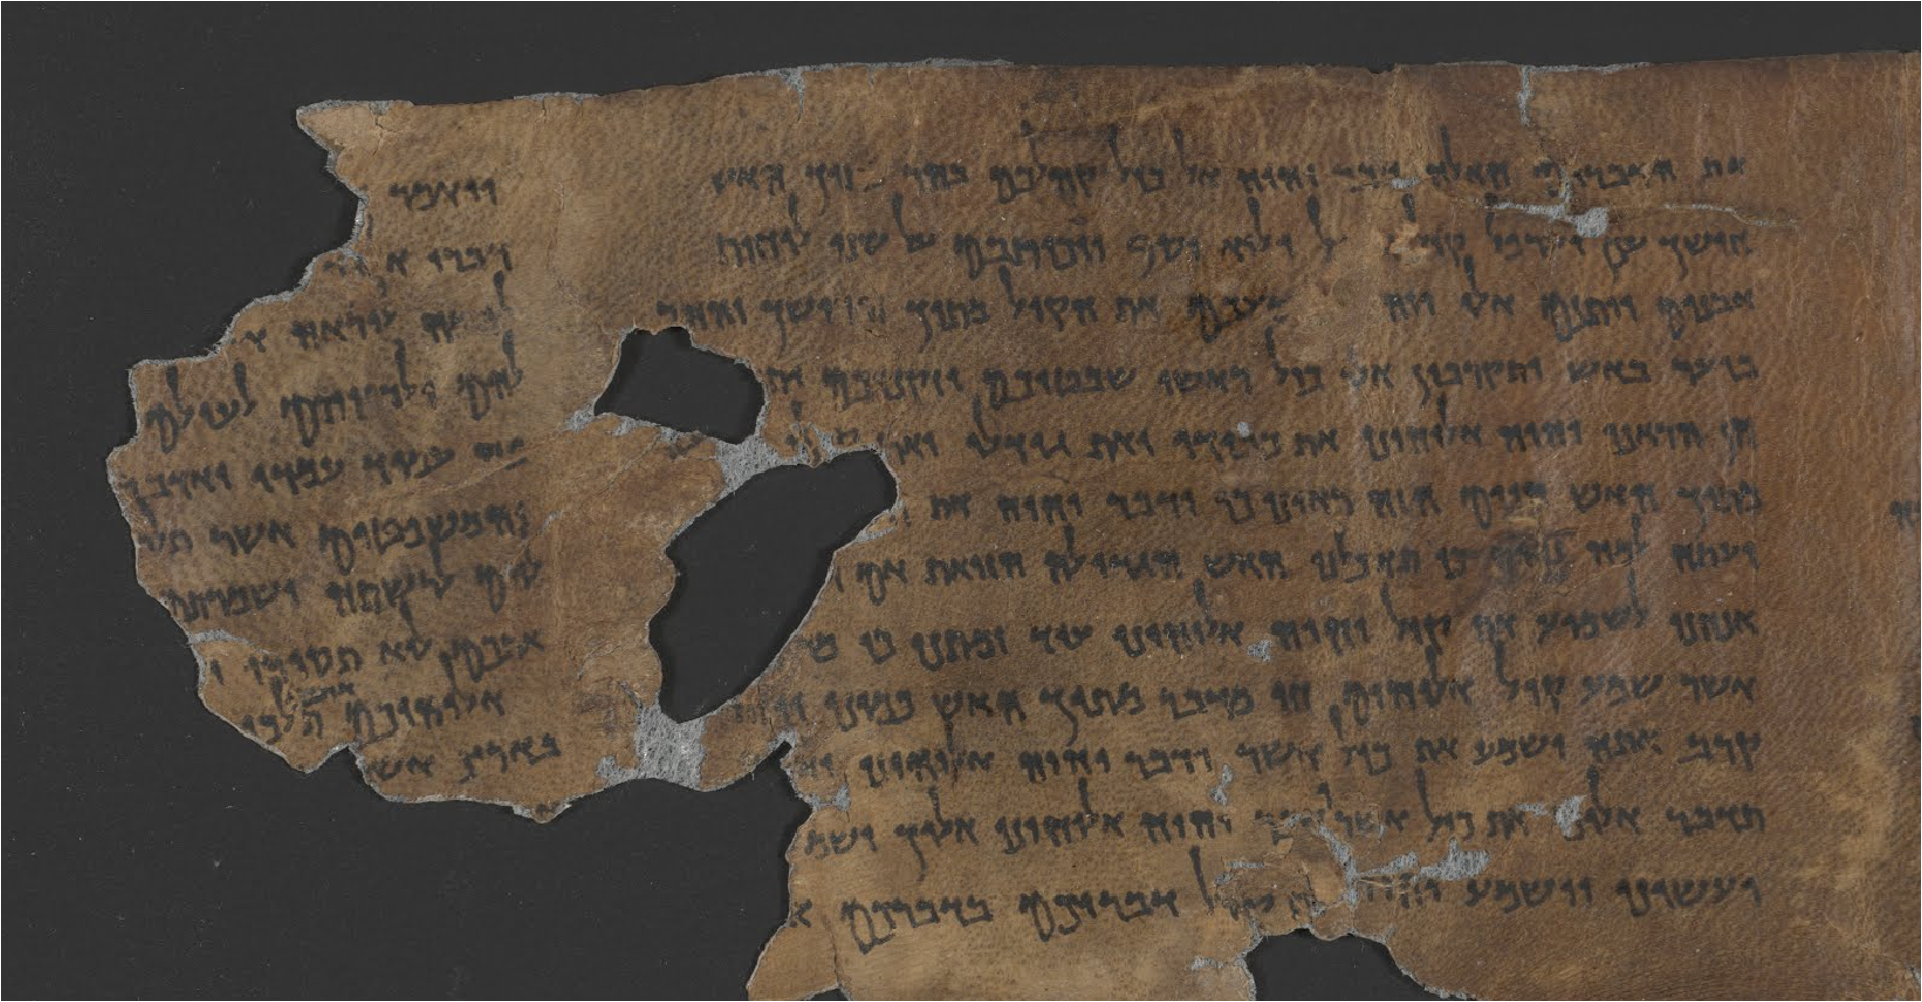
\includegraphics[width=.9\linewidth]{img/4QDt_n.png}
        \caption{4QDeut${^n}$ - Genesis}
    \end{figure}
    \tiny{Source : \href{https://www.deadseascrolls.org.il/explore-the-archive/image/B-513126}{https://www.deadseascrolls.org.il/explore-the-archive/image/B-513126}\\
    Voir encore :\\
    \begin{itemize}
        \item \href{https://www.deadseascrolls.org.il/}{https://www.deadseascrolls.org.il/}       \item\href{http://dss.collections.imj.org.il/}{http://dss.collections.imj.org.il/}
    \end{itemize}
    }
\end{frame}

\section{Le Pentateuque Samaritain}

\begin{frame}{Le Pentateuque Samaritain}
    \begin{figure}
        \centering
        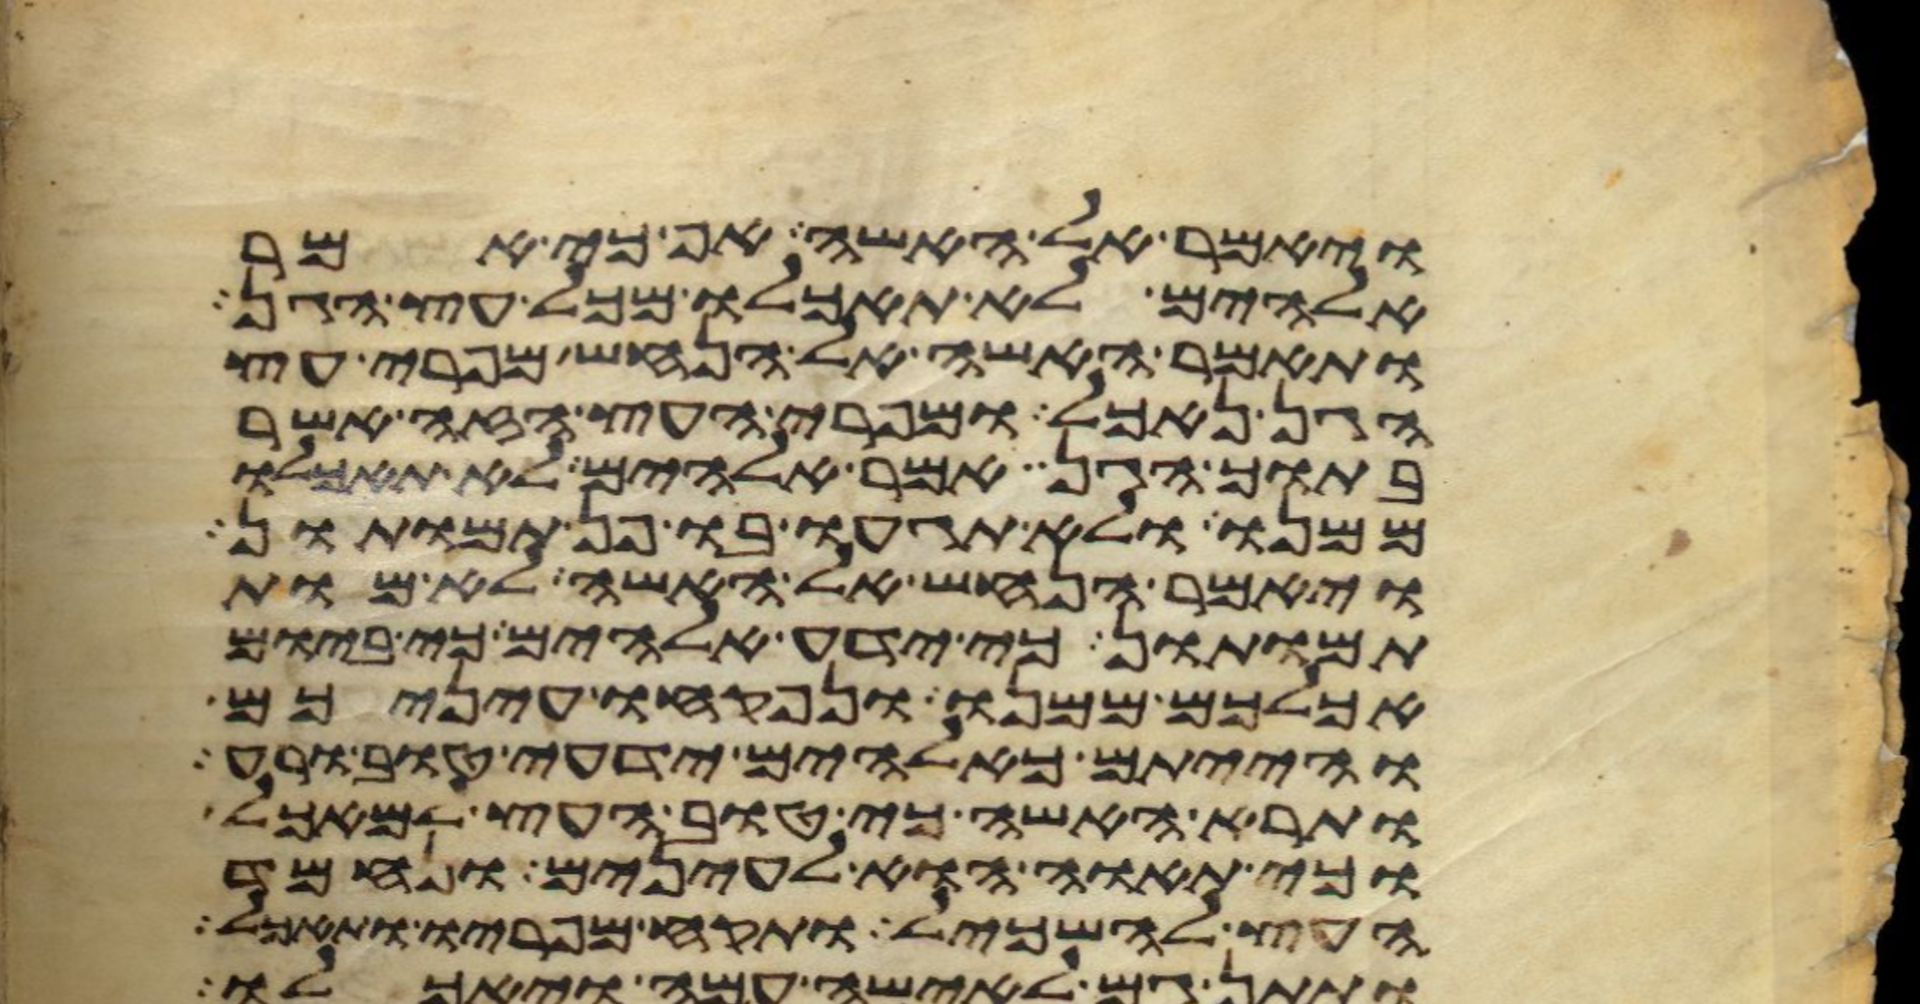
\includegraphics[width=1\linewidth]{img/chester_beatty_heb_751.png}
        \caption{Chester Beatty, Heb. 751 (1225 ap. J.-C.)}
    \end{figure}
    \tiny{Source : \href{https://viewer.cbl.ie/viewer/image/Heb_751/3/}{https://viewer.cbl.ie/viewer/image/Heb\_751/3/}\\
    Voir également : \href{https://samaritana.theologie.uni-halle.de/content/index.xml}{https://samaritana.theologie.uni-halle.de/content/index.xml}
    }
\end{frame}

\begin{frame}
\frametitle{Édition critique du Pentateuque Samaritain}
\begin{minipage}{0.48\textwidth}
    \centering
    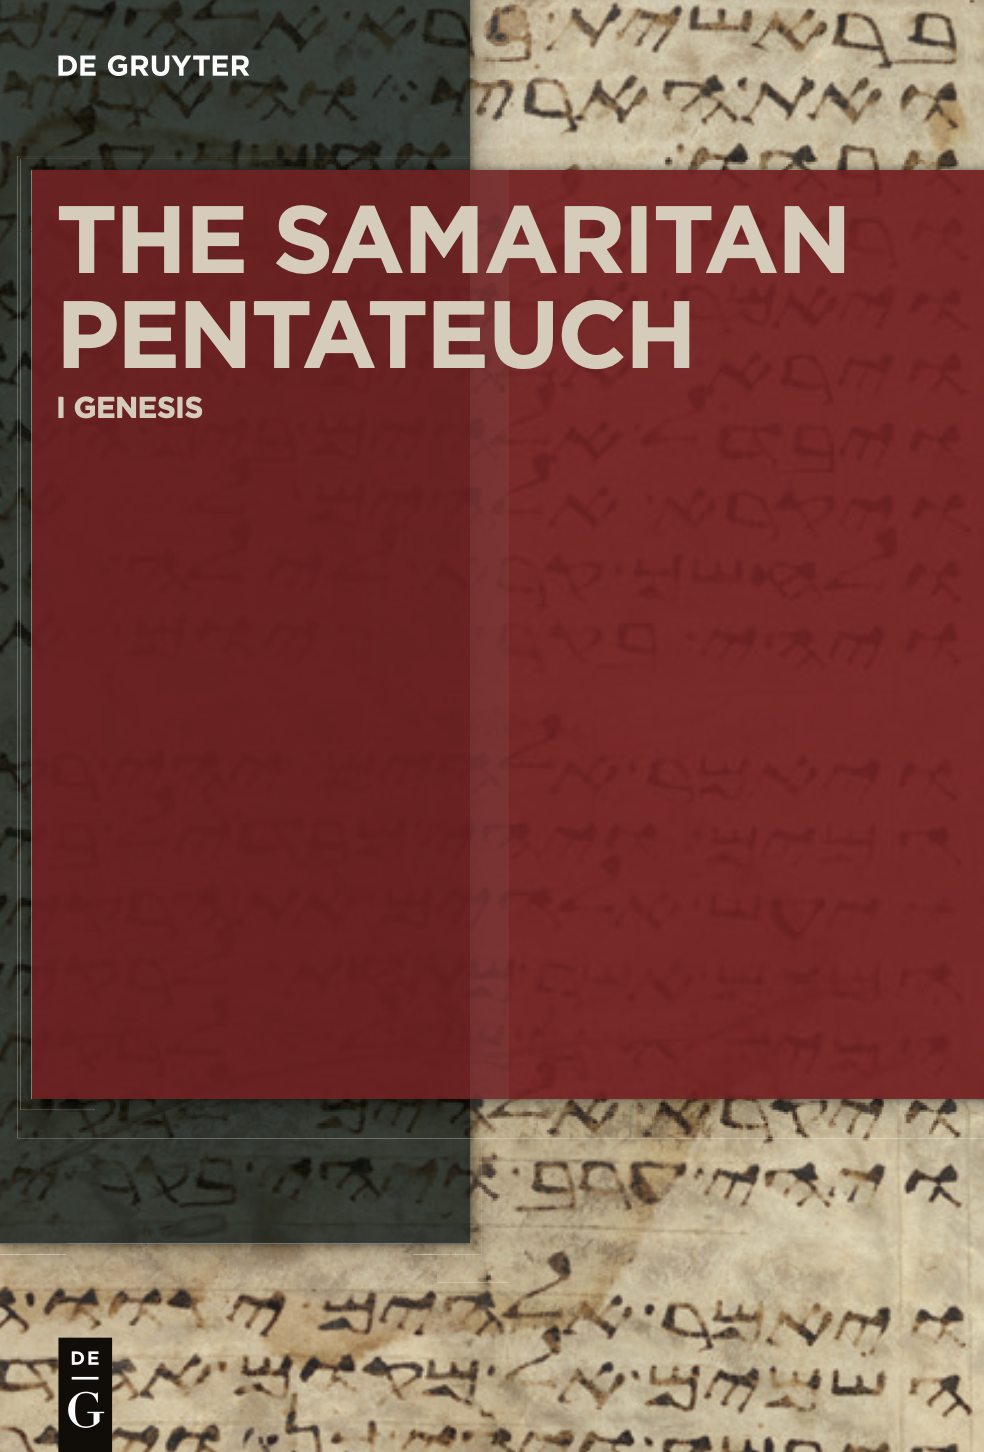
\includegraphics[width=\textwidth]{img/sam_couv.png}
\end{minipage}
\hfill
\begin{minipage}{0.48\textwidth}
    \centering
    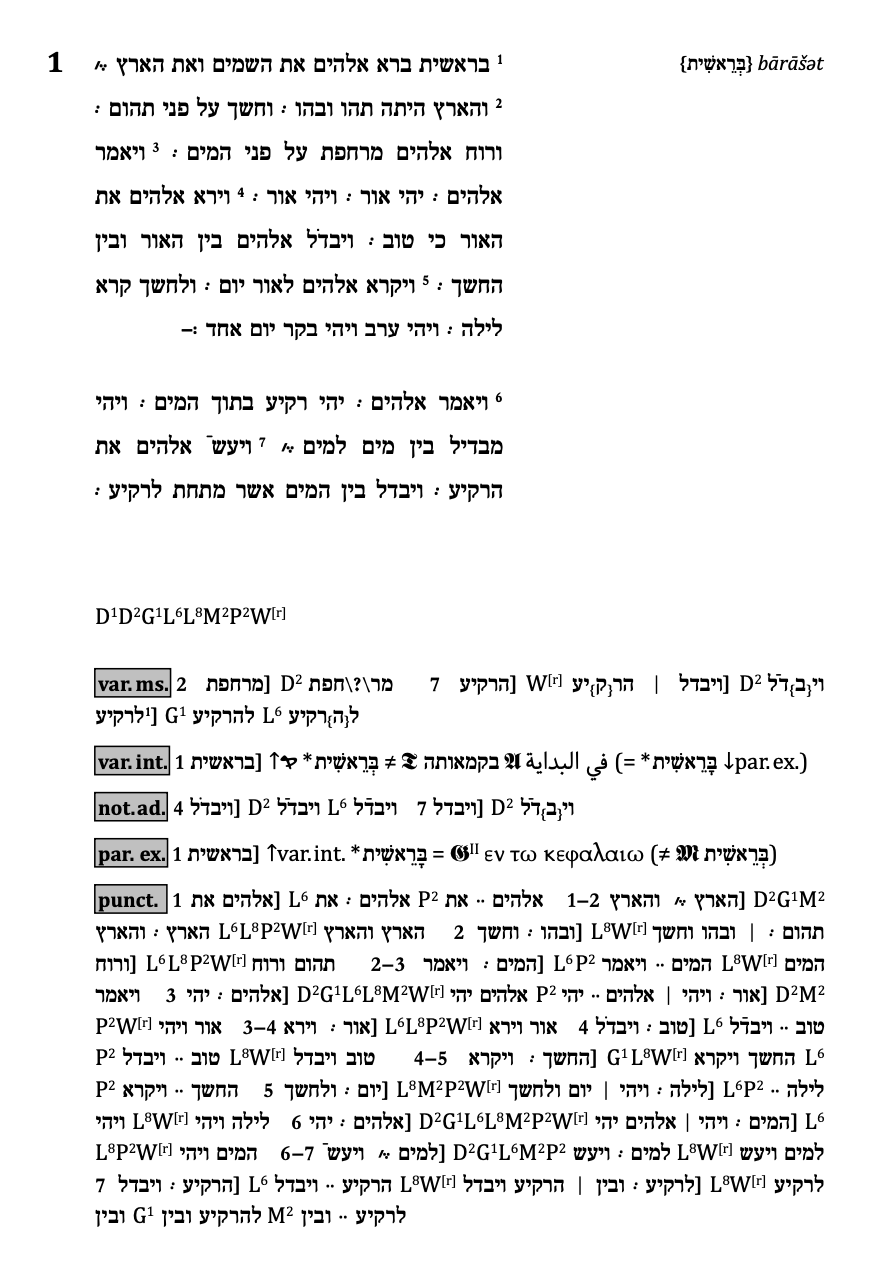
\includegraphics[width=\textwidth]{img/sam_gen_1.png}
\end{minipage}
\end{frame}

\section{Les versions grecques}
\begin{frame}{La Septante}
    \begin{figure}
        \centering
        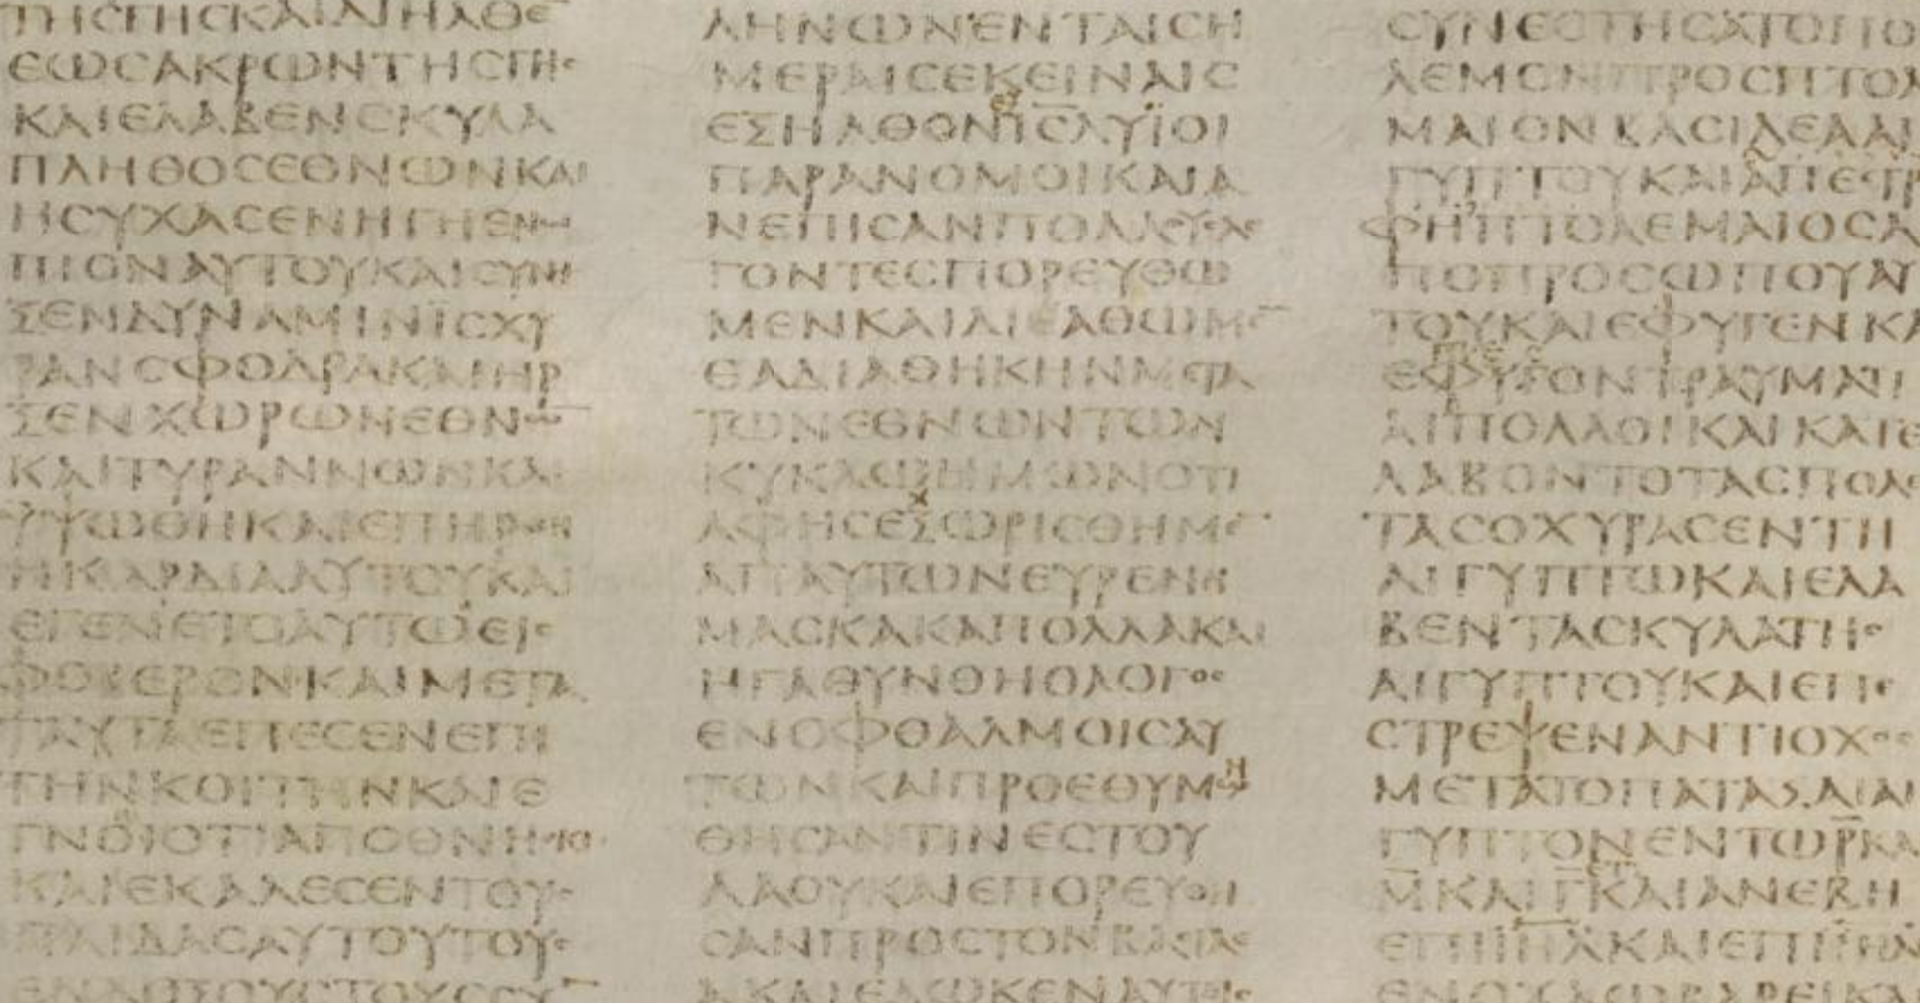
\includegraphics[width=1\linewidth]{img/Synaiticus.png}
        \caption{Codex Sinaïticus (IVe siècle)}
    \end{figure}
    \tiny{Source: \href{https://codexsinaiticus.org/en/}{https://codexsinaiticus.org/en/}}
\end{frame}


\begin{frame}{Les révisions de la Septante - les Hexaples d'Origène}
\begin{minipage}{0.48\textwidth}
    \centering
    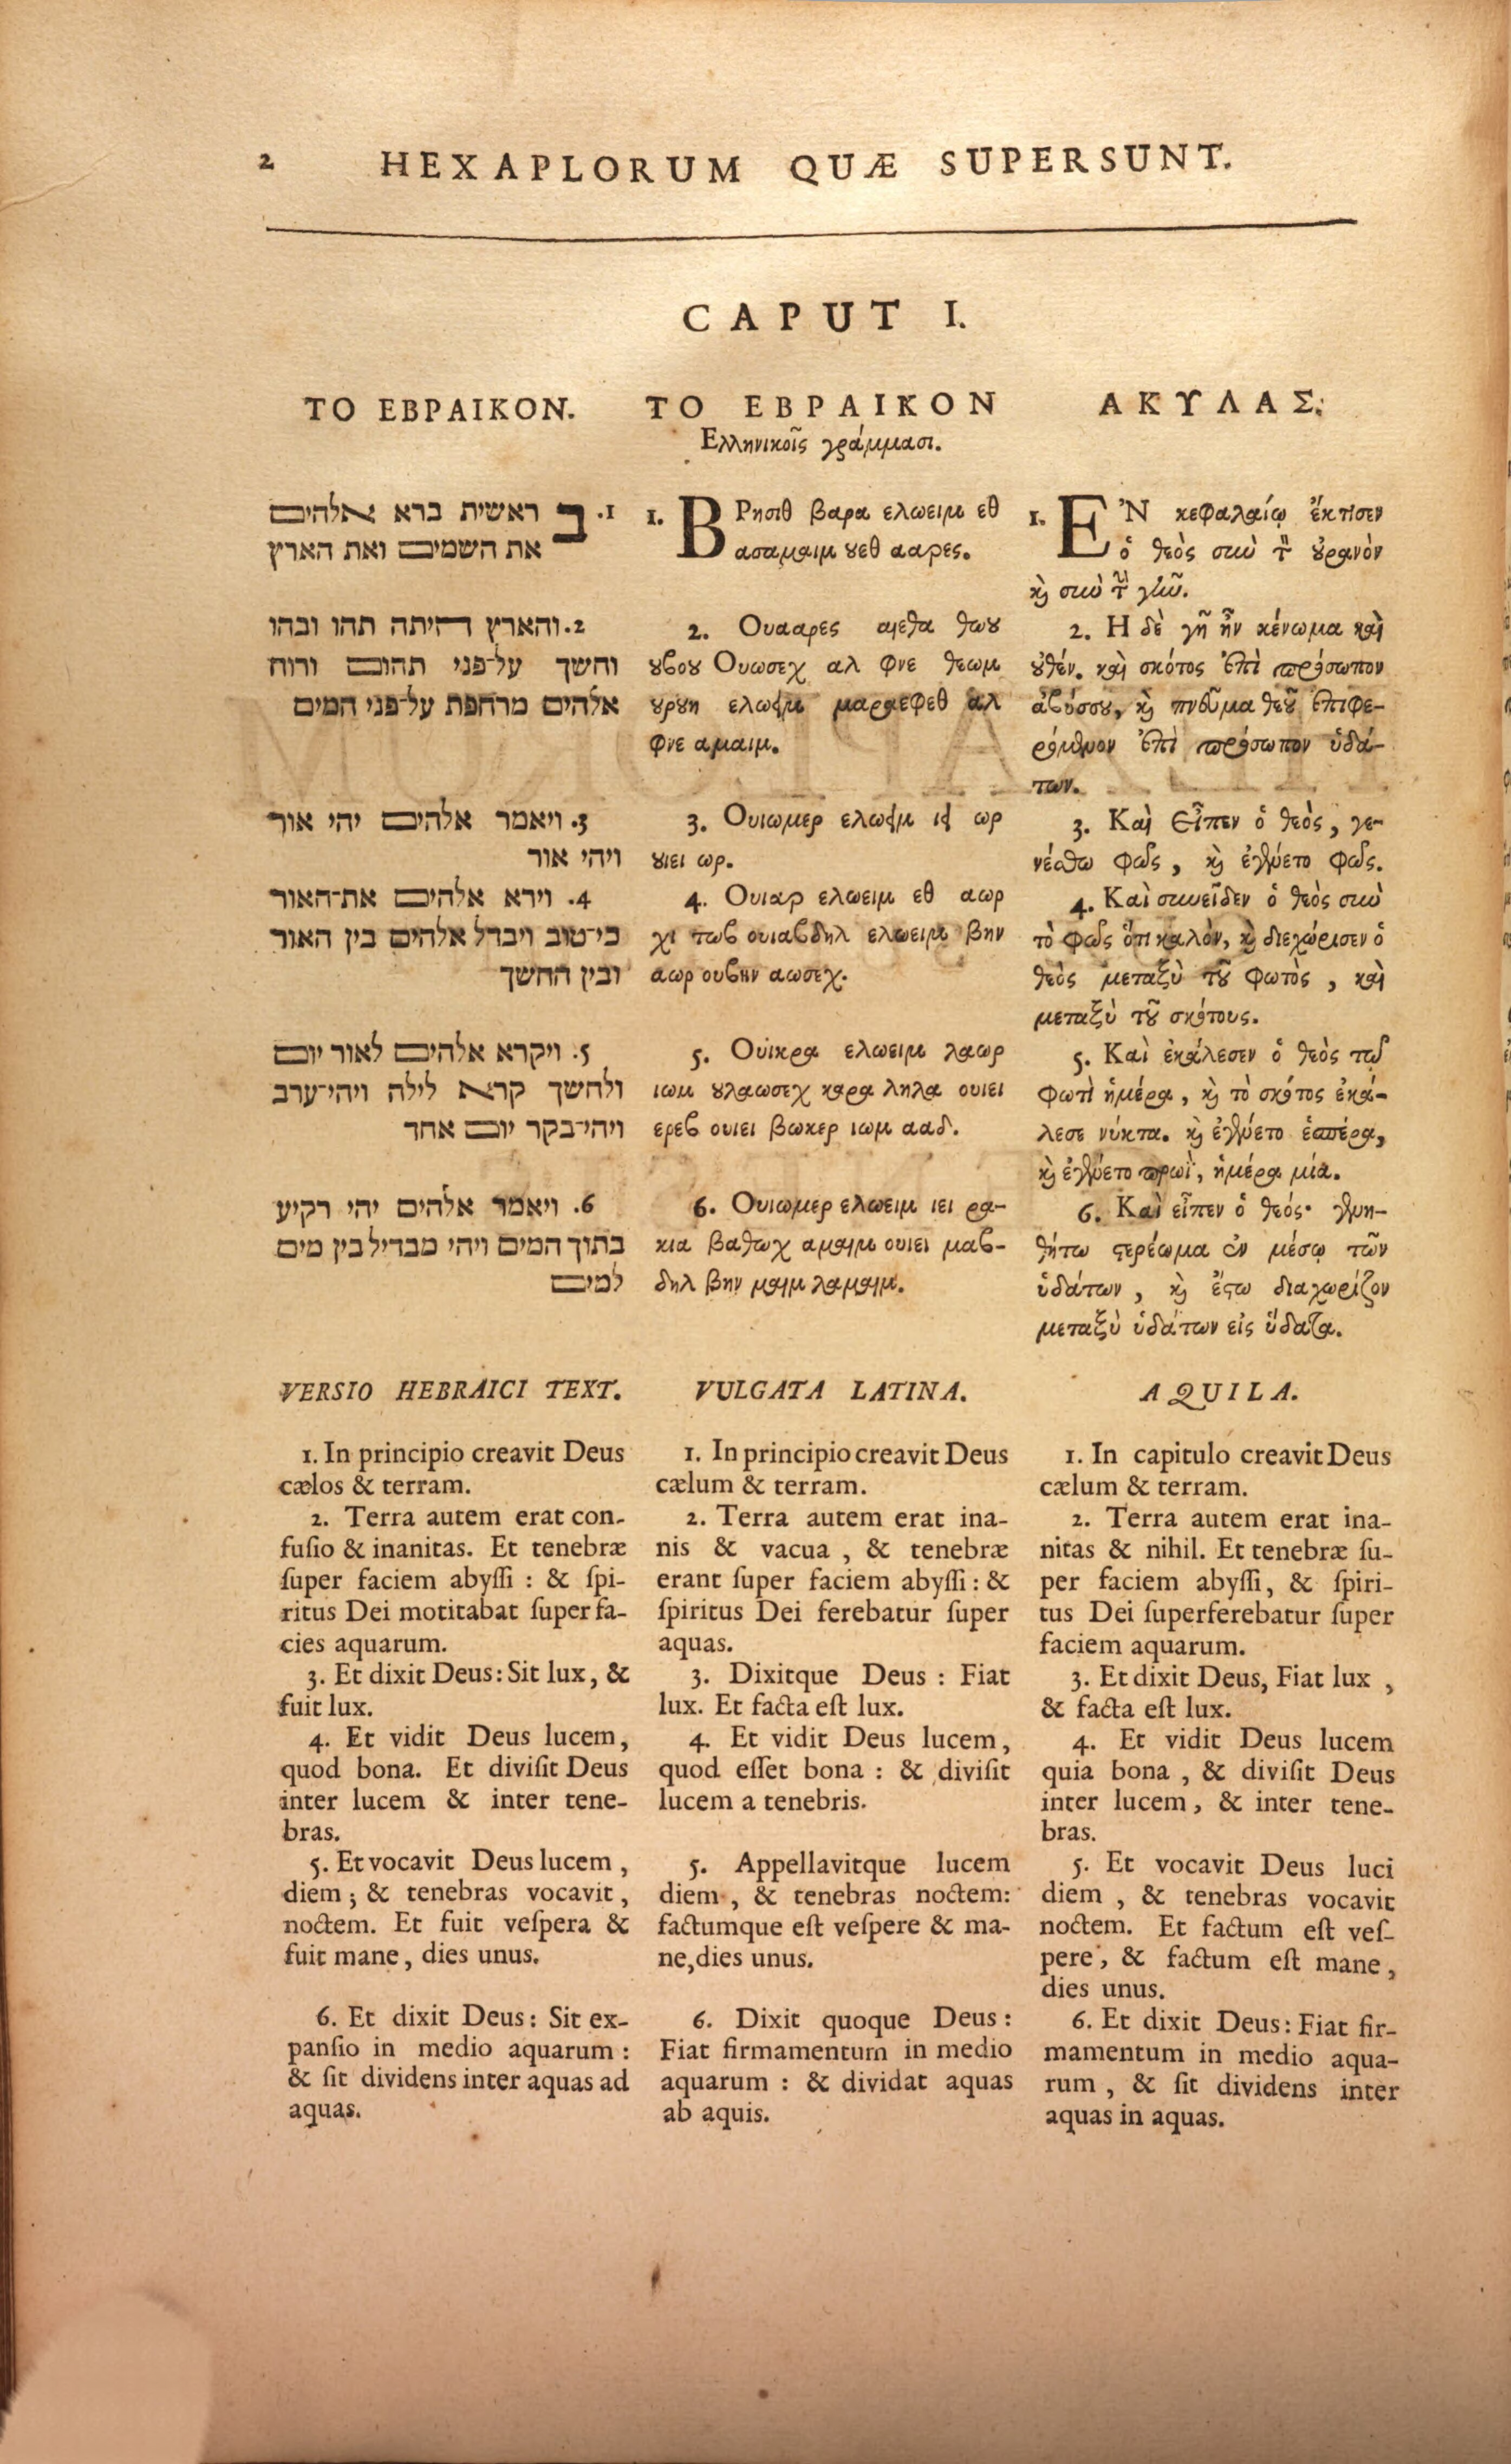
\includegraphics[width=\textwidth]{img/origen_left.jpg}
\end{minipage}
\hfill
\begin{minipage}{0.48\textwidth}
    \centering
    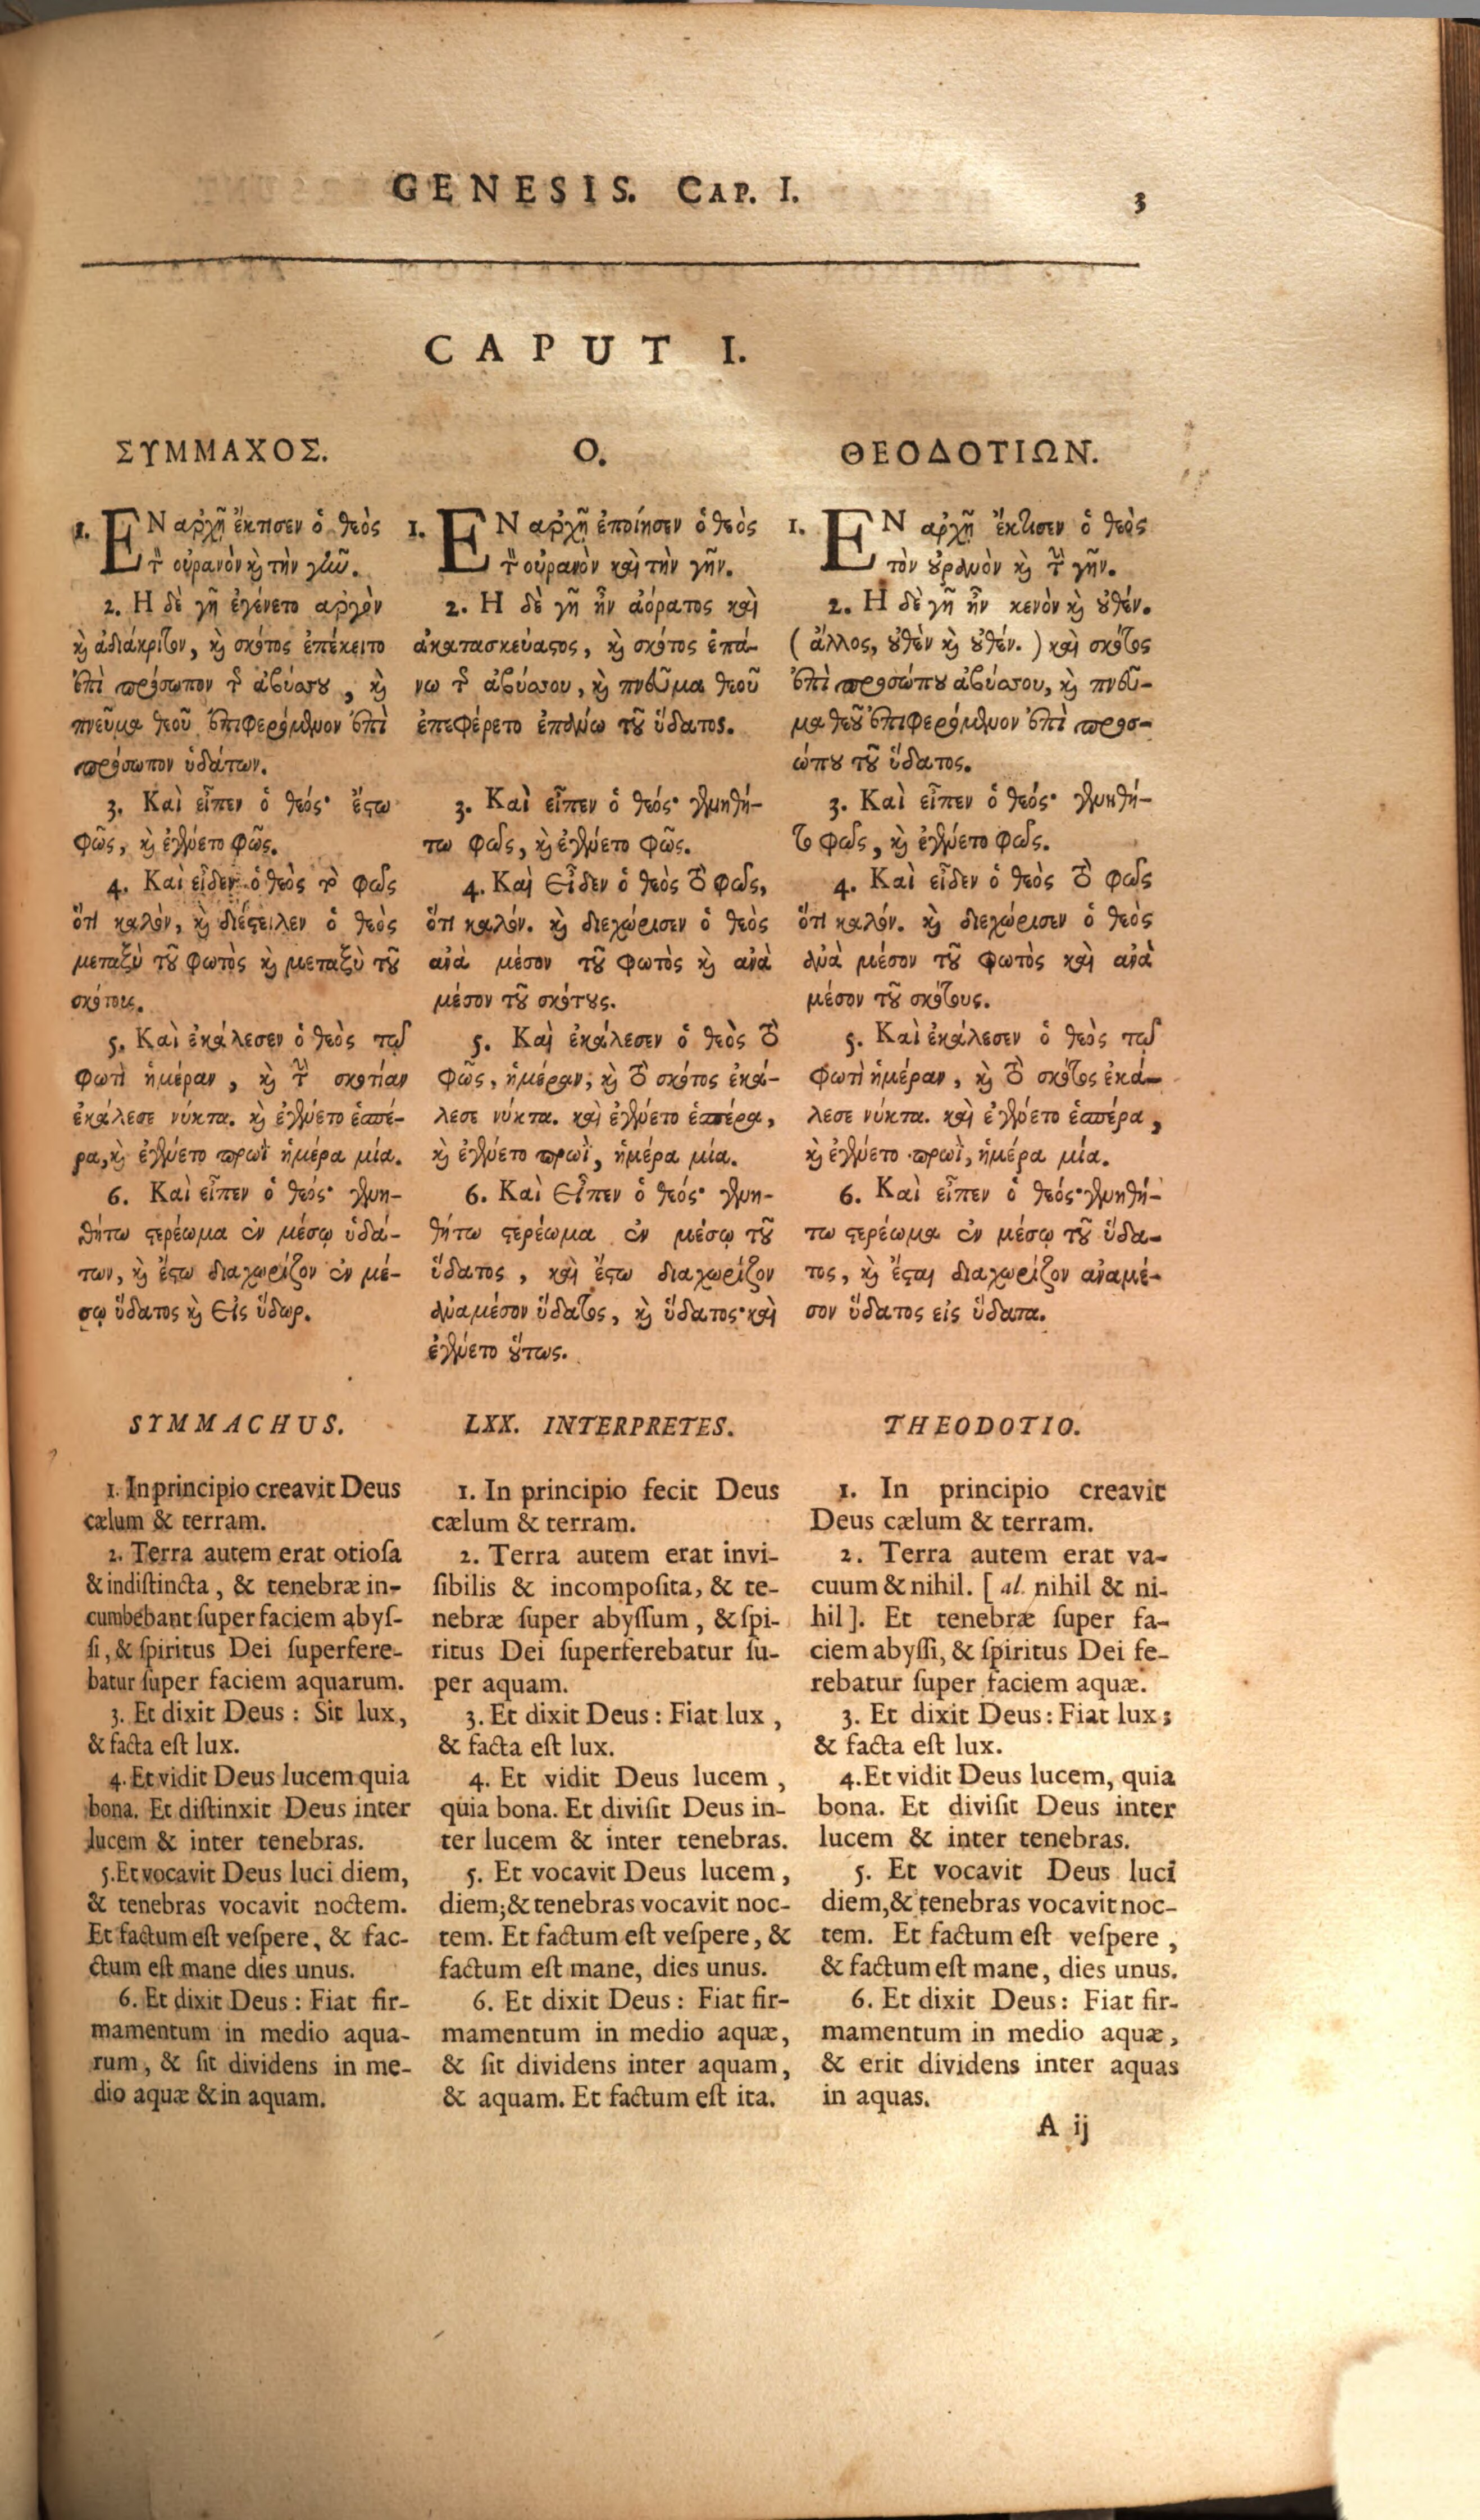
\includegraphics[width=\textwidth]{img/origen_right.jpg}
\end{minipage}
\tiny{Source: \href{https://www.digitale-sammlungen.de/en/view/bsb10212509?page=122,123}{https://www.digitale-sammlungen.de/en/view/bsb10212509?page=122,123}}
\end{frame}

\begin{frame}{Example Gen 2:23}
\begin{block}{TM}
    \texthebrew{וַיֹּאמֶר הָֽאָדָם זֹאת הַפַּעַם עֶצֶם מֵֽעֲצָמַי וּבָשָׂר מִבְּשָׂרִי לְזֹאת יִקָּרֵא אִשָּׁה כִּי מֵאִישׁ לֻֽקֳחָה־זֹּֽאת׃}
\end{block}
\begin{block}{LXX}
    \textgreek{καὶ εἶπεν Αδαμ Τοῦτο νῦν ὀστοῦν ἐκ τῶν ὀστέων μου· καὶ σὰρξ ἐκ τῆς σαρκός μου αὕτη κληθήσεται γυνή, ὅτι ἐκ τοῦ ἀνδρὸς αὐτῆς ἐλήμφθη αὕτη.}
\end{block}
\begin{block}{Révision de Symmaque}
    \textgreek{καὶ εἶπεν Αδαμ Τοῦτο νῦν ὀστοῦν ἐκ τῶν ὀστέων μου· καὶ σὰρξ ἐκ τῆς σαρκός μου αὕτη κληθήσεται \textcolor{red}{εσσα ανδρις}, ὅτι \textcolor{red}{απο ἀνδρὸς ἐλήμφθη αὕτη}.}
\end{block}
    
\end{frame}



\section{Les Targoumim, La Peshitta, La Vulgate, La Vetus Latina}
\begin{frame}{Les Targoumim et la Peshitta}
\begin{block}{Site du Comprehensive Aramaic Lexicon}
    \href{https://cal.huc.edu/}{https://cal.huc.edu/}
\end{block}
\end{frame}

\section{Les versions latines}
\begin{frame}{La Vulgate}
\begin{block}{}
    \href{http://www.perseus.tufts.edu/hopper/text?doc=Perseus%3Atext%3A1999.02.0060%3Abook%3DGenesis%3Achapter%3D1%3Averse%3D1}{http://www.perseus.tufts.edu/}}}
\end{block}
\end{frame}

\begin{frame}{La Vetus Latina}
\begin{figure}
    \centering
    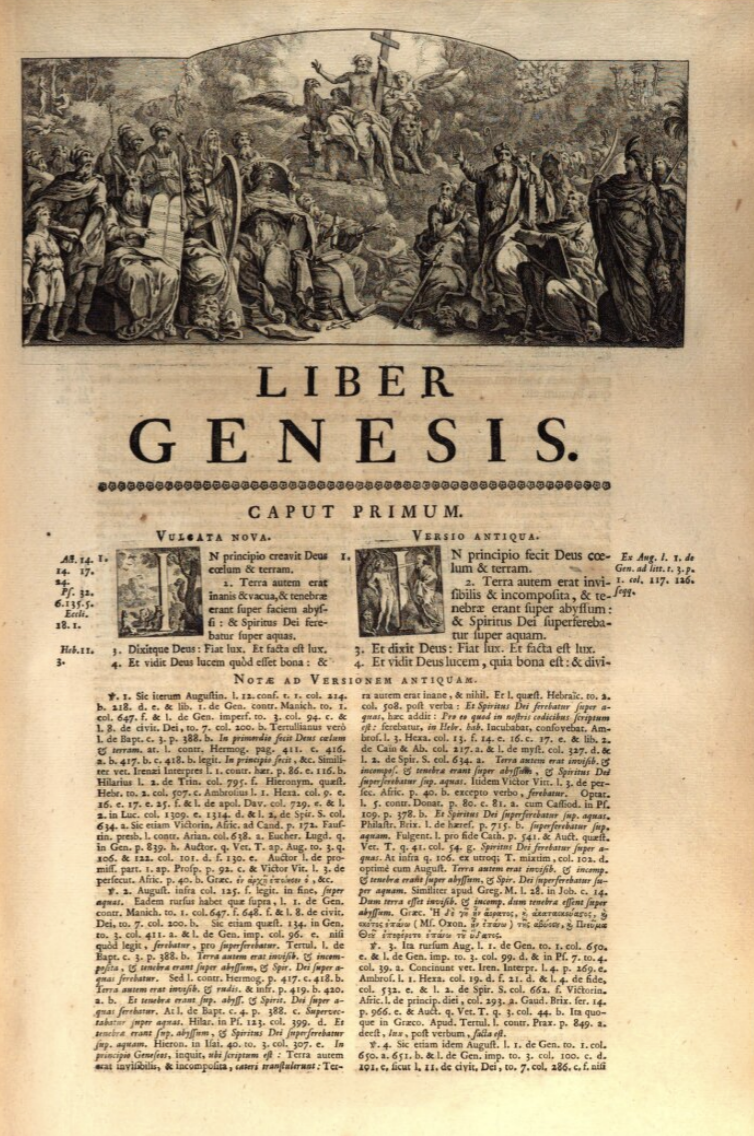
\includegraphics[width=0.5\linewidth]{img/vetus_latina_sabatier.png}
    \caption{Bibliorum sacrorum latinae versiones antiquae, seu Vetus Italica (1743)}
\end{figure}
\end{frame}
\begin{block}{}
    \href{https://www.digitale-sammlungen.de/en/view/bsb10798848?q=%28Bibliorum+sacrorum+latinae+versiones+antiquae%29&page=112,113}{https://www.digitale-sammlungen.de/}
\end{block}

\begin{frame}{Synthèse des relations entre les différents témoins}
\begin{figure}
    \centering
    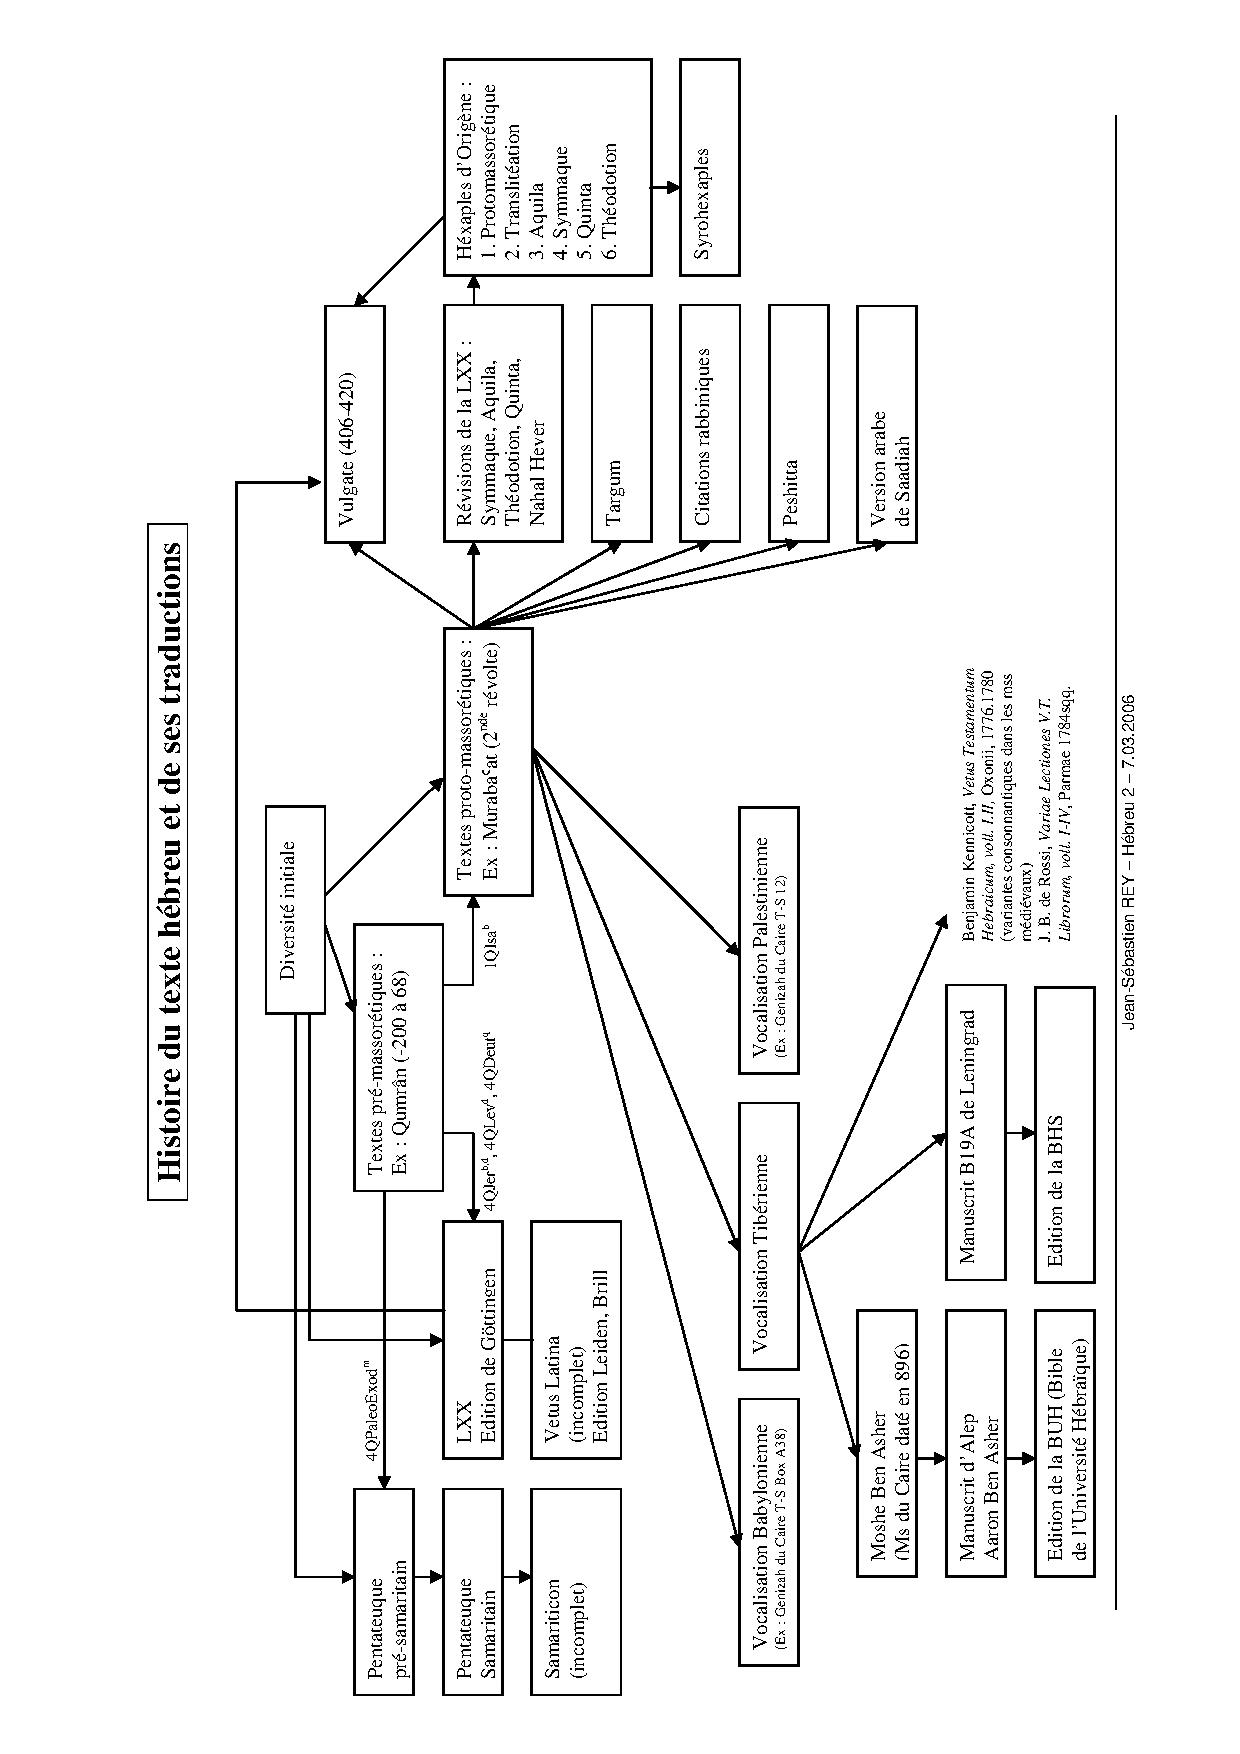
\includegraphics[width=1\linewidth]{img/Tableau histoire du texte de la bible hébraïque.jpg}
\end{figure}
    
\end{frame}
\end{document}